% CSR-MMDiff architecture figure, in the single-row style of B1's Fig. 1.
% Compiled standalone -> fig_arch.pdf; drawn at the final printed width (18.2 cm), 7 pt text.
% All sky frames and PV curves are real data of test window 2019-07-14 08:12 (scripts/arch_panels.py).
\documentclass[border=1pt]{standalone}
\usepackage{amsmath,amssymb,bm}
\usepackage{newtxtext,newtxmath}
\usepackage{tikz}
\usetikzlibrary{arrows.meta,calc,positioning}

\definecolor{imgF}{HTML}{DCE4F0}\definecolor{imgD}{HTML}{4F6FA5}
\definecolor{pvF}{HTML}{F6E3CE}\definecolor{pvD}{HTML}{9C5B2E}
\definecolor{mmF}{HTML}{EFEFEF}
\definecolor{phF}{HTML}{E3F1E0}\definecolor{phD}{HTML}{3A7D37}
\definecolor{ours}{HTML}{1F5FBF}\definecolor{spm}{HTML}{E8692F}

\begin{document}
\begin{tikzpicture}[
  font=\fontsize{7}{8.4}\selectfont,
  >={Stealth[length=3.6pt,width=3pt]},
  flow/.style={->, line width=0.55pt, draw=black!80},
  loop/.style={->, line width=0.55pt, draw=black!70, rounded corners=3pt},
  skip/.style={->, line width=0.5pt, draw=black!50, dash pattern=on 2.6pt off 1.6pt},
  iblk/.style={draw=imgD, fill=imgF, line width=0.5pt, minimum width=0.70cm, align=center, inner sep=0.5pt},
  pblk/.style={draw=pvD, fill=pvF, line width=0.5pt, minimum width=0.70cm, minimum height=0.46cm, inner sep=0.5pt},
  mma/.style={draw=black!80, fill=mmF, line width=0.5pt, minimum width=1.00cm, minimum height=0.56cm, align=center, inner sep=0.5pt},
  img/.style={inner sep=0pt, draw=black!40, line width=0.25pt},
  lbl/.style={align=center, inner sep=0.5pt},
]
\def\yI{4.06}\def\yM{2.56}\def\yP{1.00}

% ------------------------------------------------------------------ branch labels
\node[rotate=90, font=\fontsize{8}{9}\selectfont] at (0.10,\yI) {Sky images};
\node[rotate=90, font=\fontsize{8}{9}\selectfont] at (0.10,\yP) {PV power};

% ------------------------------------------------------------------ inputs
\foreach \o in {0.24,0.16,0.08}{\node[img] at (1.20+\o,\yI+\o) {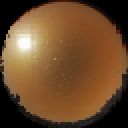
\includegraphics[width=0.95cm]{arch_ours_typical_obs_0.png}};}
\node[img] (hist) at (1.20,\yI) {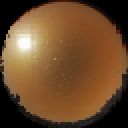
\includegraphics[width=0.95cm]{arch_ours_typical_obs_0.png}};
\node[lbl, below=2pt of hist] {history\\$\mathbf I_{t-14:t}$};
\foreach \o in {0.24,0.16,0.08}{\node[img] at (2.66+\o,\yI+\o) {
\includegraphics[width=0.95cm]{arch_noise.png}};}
\node[img] (noise) at (2.66,\yI) {
\includegraphics[width=0.95cm]{arch_noise.png}};
\node[lbl, below=2pt of noise] {noisy residual\\$\mathbf x^I_\tau$};

\node[inner sep=0pt, anchor=south west] (pvin) at (0.38,{\yP-0.52}) {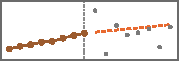
\includegraphics{arch_b1_pv_in.pdf}};
\node[lbl, anchor=south] at (1.02,{\yP+0.55}) {history};
\node[lbl, anchor=south] at (2.52,{\yP+0.55}) {\textcolor{spm}{anchor} + noisy $\mathbf x^P_\tau$};

% timestep embedding and physics prior
\node (tau) at (0.46,\yM) {$\tau$};
\node[draw=black!80, fill=white, line width=0.5pt, align=center, inner sep=1.5pt] (emb) at (1.66,\yM) {sinusoidal\\emb.\ + MLP};
\draw[flow] (tau) -- (emb);
\node[draw=phD, fill=phF, line width=0.5pt, align=center, inner sep=1.5pt] (phys) at (4.30,1.97)
  {clear-sky prior\\$P^{\mathrm{clr}}\!,\ \hat P^{\mathrm{SPM}}$};

% ------------------------------------------------------------------ coupled U-Net
\foreach \k/\r/\c/\h in {0/64/32/1.06, 1/32/64/0.82, 2/16/128/0.68, 3/8/256/0.54,
                         4/16/128/0.68, 5/32/64/0.82, 6/64/32/1.06}{
  \node[iblk, minimum height=\h cm] (I\k) at ({5.30+1.15*\k},\yI) {$\r^2$\\\c};
  \node[pblk] (P\k) at ({5.30+1.15*\k},\yP) {\c};
}
\foreach \a/\b/\s in {0/1/\downarrow,1/2/\downarrow,2/3/\downarrow,3/4/\uparrow,4/5/\uparrow,5/6/\uparrow}{
  \draw[flow] (I\a.east) -- node[above, inner sep=1.2pt] {$\s\,2$} (I\b.west);
  \draw[flow] (P\a.east) -- (P\b.west);
}
% skip connections (concatenation)
\draw[skip] (I0.north) -- (I0.north |- 0,5.02) -| (I6.north);
\draw[skip] (I1.north) -- (I1.north |- 0,4.84) -| (I5.north);
\draw[skip] (I2.north) -- (I2.north |- 0,4.66) -| (I4.north);
\draw[skip] (P0.south) -- (P0.south |- 0,0.26) -| (P6.south);
\draw[skip] (P1.south) -- (P1.south |- 0,0.43) -| (P5.south);
\draw[skip] (P2.south) -- (P2.south |- 0,0.60) -| (P4.south);
% cloud-aware RS-PV-MMA: encoder levels 2-4 and decoder level 2
\foreach \k/\w in {1/1,2/4,3/8,5/4}{
  \node[mma] (M\k) at (I\k |- 0,\yM) {CA-MMA\\$w{=}\w$};
  \draw[<->, line width=0.55pt, draw=black!80] (I\k.south) -- (M\k.north);
  \draw[<->, line width=0.55pt, draw=black!80] (M\k.south) -- (P\k.north);
}
% timestep embedding enters every block
\node[circle, draw=black!80, fill=white, line width=0.5pt, inner sep=0.8pt] (et) at (I0 |- 0,\yM) {$\mathbf e_\tau$};
\draw[flow] (emb) -- (et);
\draw[flow] (et) -- (I0.south);
\draw[flow] (et) -- (P0.north);
\node[lbl, text=black!60, anchor=west] at ($(et.north)+(0.07,0.42)$) {every\\block};

% inputs into the first blocks
\draw[flow] ($(noise.east)+(0.30,0)$) -- (I0.west);
\draw[flow] (pvin.east |- P0) -- (P0.west);
\draw[flow, draw=phD] (phys.south) -- (phys.south |- P0);
\fill[phD] (phys.south |- P0) circle (0.045);

% ------------------------------------------------------------------ projected DDIM
\node[draw=black!80, fill=mmF, line width=0.5pt, minimum width=0.64cm, minimum height=4.00cm] (ddim) at (13.25,2.62) {};
\node[rotate=90, align=center] at (ddim.center) {projected DDIM update ($\eta{=}0$)\\[1pt]
  $\mathbf x_{\tau_i}\rightarrow\mathbf x_{\tau_{i-1}}$,\; $\hat{\mathbf x}_0\in\mathcal C$};
\draw[flow] (I6.east) -- node[above, inner sep=1.2pt] {$\hat{\mathbf v}^I$} (ddim.west |- I6);
\draw[flow] (P6.east) -- node[above, inner sep=1.2pt] {$\hat{\mathbf v}^P$} (ddim.west |- P6);
% feedback loops
\draw[loop] (ddim.north) |- (2.82,5.45) -- ($(noise.north)+(0.16,0.24)$);
\node[anchor=south, inner sep=1.5pt] at (7.95,5.49) {$\mathbf x_{\tau_{i-1}}$ is fed back; $S{=}20$ steps from $\mathbf x_T\sim\mathcal N(\mathbf 0,\mathbf I)$ to $\hat{\mathbf x}_0$;\; $\mathcal C$: $0\le \hat P^{\mathrm{SPM}}+s_P\hat x^P_0\le P_{\max}$, pixels in $[-1,1]$};
\draw[loop] (ddim.south) |- (2.10,0.06) -- (2.10,{\yP-0.52});

% ------------------------------------------------------------------ outputs
\node[lbl] at (15.86,4.74) {generated $\hat{\mathbf I}$ (member 1)};
\foreach \k/\f/\l in {0/1/{+2},1/4/{+8},2/8/{+16}}{
  \node[img] (G\k) at ({14.86+\k*1.0},\yI) {\includegraphics[width=0.95cm]{arch_ours_typical_gen_\f.png}};
  \node[img] (O\k) at ({14.86+\k*1.0},2.78) {\includegraphics[width=0.95cm]{arch_ours_typical_obs_\f.png}};
  \node[lbl, below=1.5pt of O\k] {\l\ min};
}
\node[lbl] at (15.86,3.42) {observed $\mathbf I$};
\draw[flow] (ddim.east |- G0) -- (G0.west);

\node[circle, draw=ours, fill=ours!8, line width=0.5pt, inner sep=0.6pt, text=ours] (cal) at (13.98,\yP) {$s_k$};
\node[lbl, text=ours, anchor=north] at (13.98,0.80) {spread\\cal.};
\draw[flow] (ddim.east |- cal) -- (cal.west);
\node[inner sep=0pt, anchor=south west] (pvout) at (14.36,{\yP-0.51-0.36}) {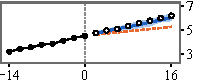
\includegraphics{arch_b1_pv_out.pdf}};
\draw[flow] (cal.east) -- (14.38,\yP);
\node[lbl] at (15.89,1.76) {calibrated PV ensemble, $M{=}30$ (kW)};

% ------------------------------------------------------------------ legend
\begin{scope}[node distance=0.10cm, lg/.style={minimum width=0.34cm, minimum height=0.22cm, inner sep=0pt, line width=0.5pt}]
  \node[lg, draw=imgD, fill=imgF] (l1) at (1.25,-0.48) {};
  \node[right=of l1] (t1) {sky-image block};
  \node[lg, draw=pvD, fill=pvF, right=0.32cm of t1] (l2) {};
  \node[right=of l2] (t2) {PV block};
  \node[lg, draw=black!80, fill=mmF, right=0.32cm of t2] (l3) {};
  \node[right=of l3] (t3) {CA-MMA (window $w$)};
  \node[lg, draw=phD, fill=phF, right=0.32cm of t3] (l4) {};
  \node[right=of l4] (t4) {physics prior};
  \coordinate[right=0.32cm of t4] (l5);
  \draw[skip] (l5) -- ++(0.50,0) coordinate (l5e);
  \node[right=0.06cm of l5e] (t5) {skip (concat.)};
  \node[right=0.32cm of t5] {$\downarrow2$\,/\,$\uparrow2$: max pool / up-sampling};
\end{scope}
\end{tikzpicture}
\end{document}
